\subsection{Translational Controller}
The translational controllers follow a cascade structure, where the velocity is the inner loop and the position is the outer loop. The relation between the controllers is presented in \autoref{fig:cascade}.\fxnote{Clarify a bit more the design, use figure 5}
%
\begin{figure}[H]
	\hspace{-.37cm}
	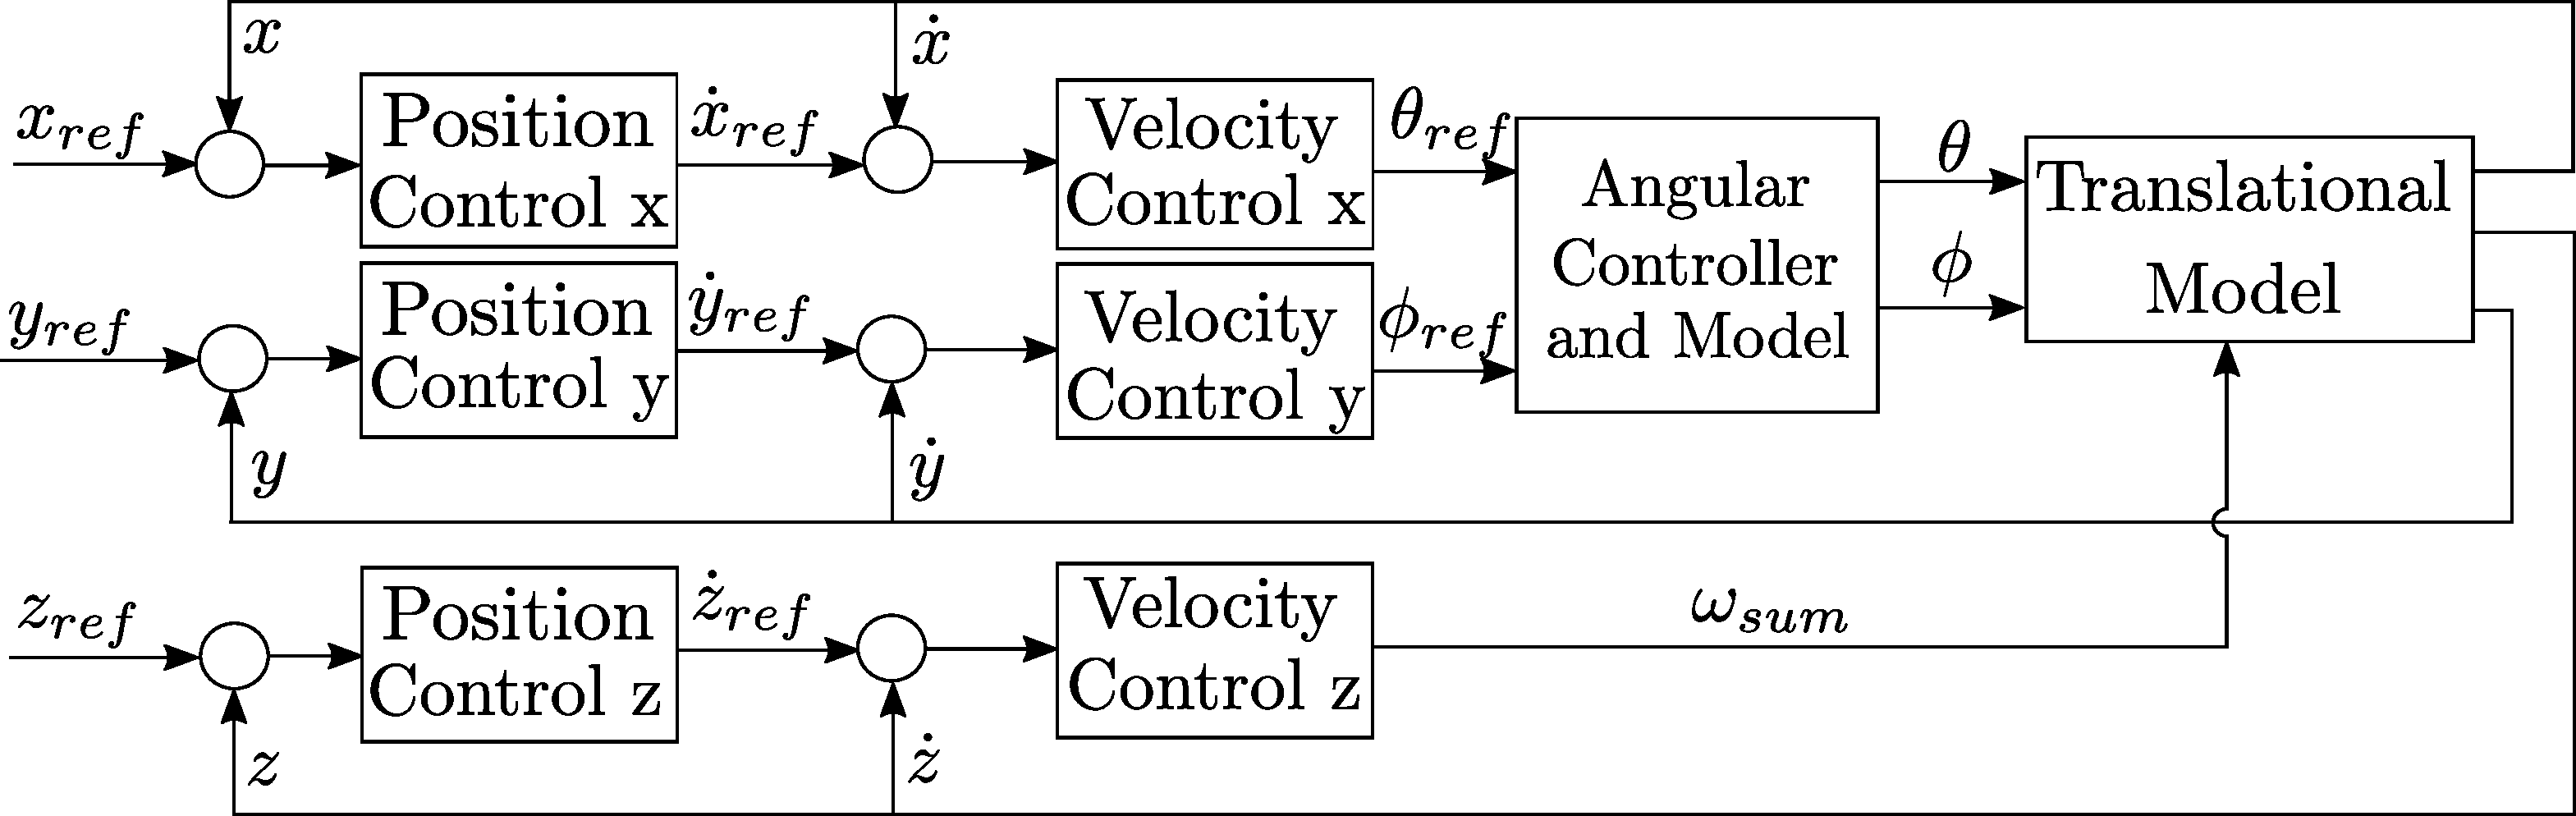
\includegraphics[width=.5\textwidth]{figures/TranslationalControlDiagram.pdf}
	\caption{Overview of translational controllers structure.}
	\label{fig:cascade}
\end{figure}
The $x_{\mathrm{I}}$ and $y_{\mathrm{I}}$ controllers share similar properties as both their outputs are angle references, $\theta_{\mathrm{ref}}$ and $\phi_{\mathrm{ref}}$. This is true as long as the system is close to the linearization point. This implies that $\psi_{\mathrm{ref}}$ is set to zero all the time, as it is desired to have zero yaw. This is done, since the translational movement can then be obtained by only rotating the other two axes. The output of the $z_{\mathrm{I}}$ controller is the required sum of motor rotational speeds.\\

To design the inner controllers for the velocities $\dot{x}_{\mathrm{I}}$, $\dot{y}_{\mathrm{I}}$ and $\dot{z}_{\mathrm{I}}$, the linear equations derived previously, see \autoref{eq:TransLinearEquations1}, \ref{eq:TransLinearEquations2} and \ref{eq:TransLinearEquations3}, are Laplace transformed. These are used to create the transfer functions, yielding
\begin{flalign}
    G_{\dot{x}}(s)&=\frac{\dot{x}_{\mathrm{I}} (s)}{\theta (s)}=\frac{-k_{\mathrm{th}} (\omega_1 ^2 + \omega_2 ^2 + \omega_3 ^2 + \omega_4 ^2)}{m s}\label{transferfunctionxdot} \\
    G_{\dot{y}}(s)&=\frac{\dot{y}_{\mathrm{I}} (s)}{\phi (s)}=\frac{k_{\mathrm{th}}(\omega_1 ^2 + \omega_2 ^2 + \omega_3 ^2 + \omega_4 ^2)}{m s}\label{transferfunctionydot} \\
    G_{\dot{z}}(s)&=\frac{\dot{z}_{\mathrm{I}}(s)}{\omega_{\mathrm{sum}}(s)} = \frac{ -2 k_{\mathrm{th}}\overline{\omega}_{\mathrm{sum}} }{ 4m s }\label{eq:linearTransferFunctionZ}
\end{flalign}

\noindent where $G_{\dot{x}}$, $G_{\dot{y}}$ and $G_{\dot{x}}$  are the plants used to design the velocity controllers in $x_{\mathrm{I}}$, $y_{\mathrm{I}}$ and $z_{\mathrm{I}}$ directions respectively,  $\dot{z}_\mathrm{I}$ is the velocity in the $z_{\mathrm{I}}$ direction, $\omega_{\mathrm{sum}}$ is the sum of the rotational speeds of the motors and $\overline{\omega}_{\mathrm{sum}}$ is the sum of the rotational speeds in equilibrium.

The three plants contain an integrator that can handle steady state errors and output disturbance. However, is there are input disturbances, which can affect the rotational speeds of the motors or external causes such as wind, an integrator term in the controller is needed for eliminating the error that they cause. Finally, a zero is then added to remove the marginal instability due to the presence of only two integrators in the system and the gain is adjusted to reduce the oscillating behavior. It is worth mentioned that, since the plants for the $x_{\mathrm{I}}$ and $z_{\mathrm{I}}$ velocities have a negative gain, the controller needs to compensate it with a negative gain as well.

Since the controllers for $\dot{x}_{\mathrm{I}}$, $\dot{y}_{\mathrm{I}}$ use the attitude controller as an inner loop to obtained the required angles, a special attention should be put on the bandwidth of the velocity controllers. If it is too fast, the inner one \fxnote{insert source, Noelia, dropbox}. Based upon a rule of thumb, which suggest a three to five times slower outer loop, the gain is designed such that the system has a bandwidth that is three times lower than the attitude control loop, which is 2 rad s$^{-1}$, to reduce the effect of its dynamic in the velocity controllers. This yields a bandwidth of around 0.7 rad s$^{-1}$ for the velocity controllers in $x_{\mathrm{I}}$ and $y_{\mathrm{I}}$ directions.

 %\cite{bandwidthReference}.

The plants of the outer loops (position control loops) contain only integrator that transforms velocity to position. Since the disturbances are handled by the inner velocity controller, a proportional controller is used. In this case, there exists an inner loop in the three axes, so the consideration of the bandwidth has to be taken into count in all of them. For $x_{\mathrm{I}}$ and $y_{\mathrm{I}}$ the final bandwidth is 0.23 rad s$^{-1}$, while for $z_{\mathrm{I}}$, is three times lower than the inner closed loop for $\dot{z}_{\mathrm{I}}$ yielding 1 rad s$^{-1}$.

%To be able to design the velocity loop for the z translational controller, the model equation derived previously, see \eqref{eq:TransLinearEquations3}, is Laplace transformed and written on the form of a transfer function, as
%%
%\vspace{-.1cm}
%%\begin{align}
%%G_{\dot{z}}=\frac{\dot{z}_{\mathrm{I}}}{\omega_{\mathrm{sum}}} &= \frac{ \frac{1}{4}(-2 k_{\mathrm{th}})\overline{\omega}_{\mathrm{sum}} }{ m s }\label{eq:linearTransferFunctionZ}
%%\end{align}
%
%%\noindent where $\dot{z}_\mathrm{I}$ is the velocity in the $z_{\mathrm{I}}$ direction, $\omega_{\mathrm{sum}}$ is the sum of the rotational speeds of the motors and $\overline{\omega}_{\mathrm{sum}}$ is the sum of the rotational speeds in equilibrium.
%
%Due to an integrator and a negative gain, the system's root locus moves into the right half plane as the gain increases. A proportional controller with negative gain ensures the system to be stable. 
%
%As there is not an inner control loop, input disturbances may occur such that a steady state error appears, which is not eliminated by the integrator in the plant. To remove this potential error an integrator term is added, leading to a PI-controller. 
%
%The plant for the z position controller is just an integrator and a proportional controller is utilized. This is as well designed so that the bandwidth is three times lower than the inner one.
